% Our GFM schematic: multimodal inputs -> frozen TerraMind ViT -> embedding space -> downstream tasks (soil moisture = this work).
% Compile: pdflatex gfm_embedding_schematic.tex ; PNG: gs -sDEVICE=png16m -r300 -o gfm_embedding_schematic.png gfm_embedding_schematic.pdf
\documentclass{article}
\usepackage[paperwidth=34.0cm,paperheight=12.7cm,margin=0pt]{geometry}
\usepackage{amssymb}
\pagestyle{empty}
\setlength{\parindent}{0pt}
\usepackage{mathptmx}
\usepackage{tikz}
\usetikzlibrary{arrows.meta,calc,positioning,shapes.geometric}

% palette H
\definecolor{dblue}{HTML}{08519C}
\definecolor{lblue}{HTML}{6BAED6}
\definecolor{orng}{HTML}{E6550D}
\definecolor{dgrey}{HTML}{525252}
% imagery colours
\definecolor{vegA}{HTML}{2E7D32}
\definecolor{vegB}{HTML}{C8B88A}
\definecolor{sarA}{HTML}{1A1A1A}
\definecolor{sarB}{HTML}{E0E0E0}
\definecolor{demA}{HTML}{4E8F5A}
\definecolor{demB}{HTML}{B5835A}

% \mosaic{x}{y}{size}{colA}{colB}{seed}: 8x8 random pixel tile, shades between colA and colB
\newcommand{\mosaic}[6]{%
  \pgfmathsetseed{#6}%
  \foreach \i in {0,...,7}{\foreach \j in {0,...,7}{%
    \pgfmathtruncatemacro{\p}{100*rnd}%
    \fill[#4!\p!#5] ({#1+\i*#3/8},{#2+\j*#3/8}) rectangle ++({#3/8},{#3/8});}}%
  \draw[black,line width=0.9pt] (#1,#2) rectangle ++(#3,#3);}

% \stack{x}{y}{size}{n}{fill}: n offset back layers behind a tile
\newcommand{\stack}[5]{%
  \foreach \k in {#4,...,1}{%
    \filldraw[fill=#5,draw=black,line width=0.6pt] ({#1+0.13*\k},{#2+0.13*\k}) rectangle ++(#3,#3);}}

% \cluster{cx}{cy}{colour}{seed}: 14 points around a centre
\newcommand{\cluster}[4]{%
  \pgfmathsetseed{#4}%
  \foreach \n in {1,...,14}{%
    \pgfmathsetmacro{\dx}{0.55*(rnd-0.5)+0.35*(rnd-0.5)}%
    \pgfmathsetmacro{\dy}{0.55*(rnd-0.5)+0.35*(rnd-0.5)}%
    \fill[#3,draw=black,line width=0.3pt] ({#1+\dx},{#2+\dy}) circle (0.075);}}

\begin{document}
\vspace*{0.4cm}\hspace*{0.45cm}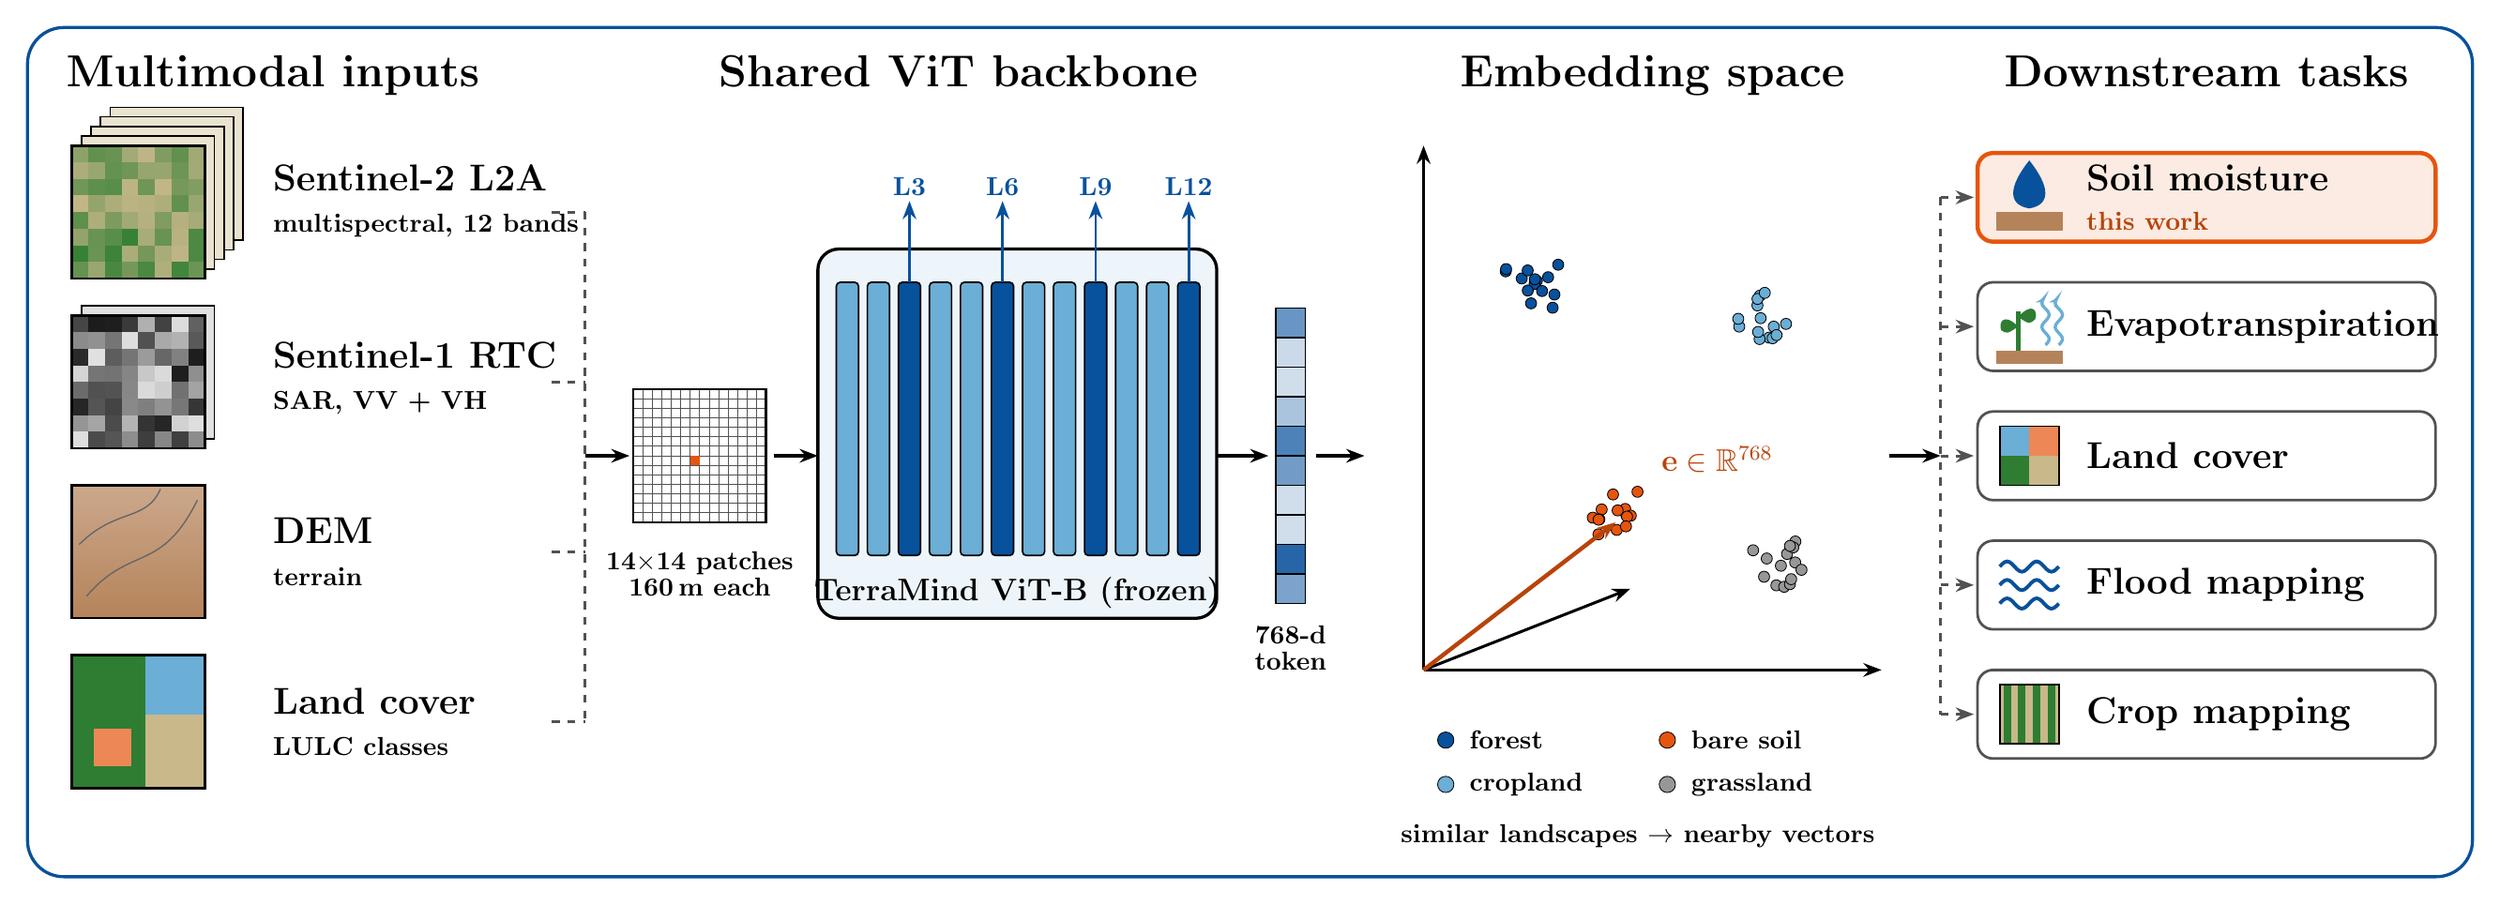
\begin{tikzpicture}[font=\bfseries\Large, >={Stealth[length=7pt]}]

%---------------- outer frame
\draw[rounded corners=14pt, line width=1.2pt, dblue] (-0.6,-0.9) rectangle (32.5,10.6);

%---------------- column headers
\node[anchor=base west, font=\bfseries\LARGE] at (-0.2,9.8) {Multimodal inputs};
\node[anchor=base, font=\bfseries\LARGE] at (12.0,9.8) {Shared ViT backbone};
\node[anchor=base, font=\bfseries\LARGE] at (21.4,9.8) {Embedding space};
\node[anchor=base, font=\bfseries\LARGE] at (28.9,9.8) {Downstream tasks};

%---------------- inputs (one tile per modality)
% S2
\stack{0}{7.2}{1.8}{4}{vegB!40}
\mosaic{0}{7.2}{1.8}{vegA}{vegB}{11}
\node[anchor=west, align=left] at (2.6,8.25) {Sentinel-2 L2A\\[-2pt]{\normalsize multispectral, 12 bands}};
% S1
\stack{0}{4.9}{1.8}{1}{sarB}
\mosaic{0}{4.9}{1.8}{sarA}{sarB}{23}
\node[anchor=west, align=left] at (2.6,5.85) {Sentinel-1 RTC\\[-2pt]{\normalsize SAR, VV + VH}};
% DEM (smooth)
\shade[left color=demA, right color=demB, top color=demB!70!white] (0,2.6) rectangle ++(1.8,1.8);
\draw[black!60, line width=0.5pt] (0.2,2.9) .. controls (0.8,3.6) and (1.2,3.2) .. (1.7,4.2);
\draw[black!60, line width=0.5pt] (0.1,3.6) .. controls (0.6,4.1) and (1.0,3.9) .. (1.2,4.35);
\draw[black, line width=0.9pt] (0,2.6) rectangle ++(1.8,1.8);
\node[anchor=west, align=left] at (2.6,3.5) {DEM\\[-2pt]{\normalsize terrain}};
% LULC (categorical blocks)
\fill[vegA]  (0,0.3) rectangle (1.0,2.1);
\fill[vegB]  (1.0,0.3) rectangle (1.8,1.3);
\fill[lblue] (1.0,1.3) rectangle (1.8,2.1);
\fill[orng!70] (0.3,0.6) rectangle (0.8,1.1);
\draw[black, line width=0.9pt] (0,0.3) rectangle ++(1.8,1.8);
\node[anchor=west, align=left] at (2.6,1.2) {Land cover\\[-2pt]{\normalsize LULC classes}};

%---------------- patchify
\coordinate (P) at (7.6,3.9);
\fill[white] (P) rectangle ++(1.8,1.8);
\foreach \t in {0,...,14}{
  \draw[dgrey, line width=0.35pt] ($(P)+(\t*1.8/14,0)$) -- ++(0,1.8);
  \draw[dgrey, line width=0.35pt] ($(P)+(0,\t*1.8/14)$) -- ++(1.8,0);}
\fill[orng] ($(P)+(6*1.8/14,6*1.8/14)$) rectangle ++(1.8/14,1.8/14);
\draw[black, line width=0.9pt] (P) rectangle ++(1.8,1.8);
\node[align=center, font=\bfseries\normalsize] at (8.5,3.2) {14$\times$14 patches\\[-2pt]160\,m each};

\foreach \y in {8.1,5.8,3.5,1.2}
  \draw[dashed, line width=1.1pt, dgrey] (6.5,\y) -- (6.95,\y);
\draw[dashed, line width=1.1pt, dgrey] (6.95,8.1) -- (6.95,1.2);
\draw[->, line width=1.4pt] (6.95,4.8) -- (7.55,4.8);

%---------------- ViT backbone (12 blocks, taps at L3 L6 L9 L12)
\draw[rounded corners=8pt, line width=1.2pt, fill=lblue!12] (10.1,2.6) rectangle (15.5,7.6);
\node[font=\bfseries\large] at (12.8,2.95) {TerraMind ViT-B (frozen)};
\foreach \b in {1,...,12}{
  \pgfmathsetmacro{\xx}{10.35+(\b-1)*0.42}
  \ifnum\b=3 \def\bc{dblue}\else\ifnum\b=6 \def\bc{dblue}\else\ifnum\b=9 \def\bc{dblue}\else\ifnum\b=12 \def\bc{dblue}\else\def\bc{lblue}\fi\fi\fi\fi
  \filldraw[fill=\bc, draw=black, line width=0.6pt, rounded corners=1.5pt] (\xx,3.45) rectangle ++(0.3,3.7);
}
\foreach \b in {3,6,9,12}{
  \pgfmathsetmacro{\xx}{10.35+(\b-1)*0.42+0.15}
  \draw[->, line width=1pt, dblue] (\xx,7.15) -- (\xx,8.25);
  \node[font=\bfseries\normalsize, dblue, above] at (\xx,8.2) {L\b};
}
\draw[->, line width=1.4pt] (9.5,4.8) -- (10.1,4.8);

%---------------- token vector
\draw[->, line width=1.4pt] (15.5,4.8) -- (16.2,4.8);
\pgfmathsetseed{5}
\foreach \c in {0,...,9}{
  \pgfmathtruncatemacro{\p}{15+80*rnd}
  \filldraw[fill=dblue!\p!white, draw=black, line width=0.5pt] (16.3,{2.8+\c*0.4}) rectangle ++(0.4,0.4);}
\node[font=\bfseries\normalsize, align=center] at (16.5,2.2) {768-d\\[-2pt]token};
\draw[->, line width=1.4pt] (16.85,4.8) -- (17.5,4.8);

%---------------- embedding space (3-D axes + landscape clusters)
\coordinate (O) at (18.3,1.9);
\draw[->, line width=1.1pt] (O) -- ++(6.2,0);
\draw[->, line width=1.1pt] (O) -- ++(0,7.1);
\draw[->, line width=1.1pt] (O) -- ++(2.8,1.1);
\cluster{19.7}{7.0}{dblue}{3}
\cluster{22.9}{6.6}{lblue}{7}
\cluster{20.9}{3.9}{orng}{13}
\cluster{23.2}{3.4}{dgrey!60}{17}
\draw[->, line width=1.6pt, orng!80!black] (O) -- (20.9,3.9);
\node[font=\bfseries\large, orng!80!black, anchor=west] at (21.4,4.75) {$\mathbf{e}\in\mathbb{R}^{768}$};
% legend
\foreach \col/\lab/\yy in {dblue/forest/0.95, lblue/cropland/0.35}{
  \fill[\col,draw=black,line width=0.3pt] (18.6,\yy) circle (0.11);
  \node[anchor=west, font=\bfseries\normalsize] at (18.8,\yy) {\lab};}
\foreach \col/\lab/\yy in {orng/bare soil/0.95, dgrey!60/grassland/0.35}{
  \fill[\col,draw=black,line width=0.3pt] (21.6,\yy) circle (0.11);
  \node[anchor=west, font=\bfseries\normalsize] at (21.8,\yy) {\lab};}
\node[font=\bfseries\normalsize, align=center] at (21.2,-0.35) {similar landscapes $\rightarrow$ nearby vectors};

%---------------- downstream tasks (bus from the embedding space, one box per task)
\draw[->, line width=1.4pt] (24.6,4.8) -- (25.3,4.8);
\draw[dashed, line width=1.1pt, dgrey] (25.3,8.3) -- (25.3,1.3);
\foreach \y in {8.3,6.55,4.8,3.05,1.3}
  \draw[->, dashed, line width=1.1pt, dgrey] (25.3,\y) -- (25.75,\y);
% boxes
\filldraw[fill=orng!12, draw=orng, line width=1.6pt, rounded corners=6pt] (25.8,7.7) rectangle (32.0,8.9);
\foreach \y in {6.55,4.8,3.05,1.3}
  \filldraw[fill=white, draw=dgrey, line width=1pt, rounded corners=6pt] (25.8,{\y-0.6}) rectangle (32.0,{\y+0.6});
% icons (centred at x = 26.5)
% soil moisture: droplet over soil
\fill[demB] (26.05,7.85) rectangle (26.95,8.1);
\fill[dblue] (26.5,8.8) .. controls (26.78,8.45) and (26.8,8.2) .. (26.5,8.15) .. controls (26.2,8.2) and (26.22,8.45) .. (26.5,8.8);
% evapotranspiration: plant with rising vapour
\fill[demB] (26.05,6.05) rectangle (26.95,6.22);
\draw[vegA, line width=1.6pt] (26.35,6.22) -- (26.35,6.75);
\fill[vegA] (26.35,6.55) .. controls (26.15,6.75) and (26.08,6.6) .. (26.12,6.5) .. controls (26.2,6.45) .. (26.35,6.55);
\fill[vegA] (26.35,6.68) .. controls (26.55,6.9) and (26.62,6.75) .. (26.58,6.65) .. controls (26.5,6.58) .. (26.35,6.68);
\foreach \xo in {26.72,26.9}
  \draw[->, lblue, line width=1.2pt, >={Stealth[length=4pt]}] plot[domain=0:0.65, samples=20] ({\xo+0.05*sin(\x*1100)},{6.3+\x});
% land cover: four classes
\fill[vegA] (26.1,4.4) rectangle (26.5,4.8); \fill[vegB] (26.5,4.4) rectangle (26.9,4.8);
\fill[lblue] (26.1,4.8) rectangle (26.5,5.2); \fill[orng!70] (26.5,4.8) rectangle (26.9,5.2);
\draw[black, line width=0.6pt] (26.1,4.4) rectangle (26.9,5.2);
% flood: waves
\foreach \o in {0.25,0,-0.25}
  \draw[dblue, line width=1.4pt] plot[domain=0:0.8, samples=25] ({26.1+\x},{3.05+\o+0.07*sin(\x*900)});
% crops: field rows
\fill[vegB] (26.1,0.9) rectangle (26.9,1.7);
\foreach \r in {0,1,2,3}
  \fill[vegA] ({26.15+\r*0.2},0.9) rectangle ++(0.1,0.8);
\draw[black, line width=0.6pt] (26.1,0.9) rectangle (26.9,1.7);
% labels
\node[anchor=west, align=left] at (27.15,8.3) {Soil moisture\\[-3pt]{\normalsize\textcolor{orng!80!black}{this work}}};
\node[anchor=west] at (27.15,6.55) {Evapotranspiration};
\node[anchor=west] at (27.15,4.8) {Land cover};
\node[anchor=west] at (27.15,3.05) {Flood mapping};
\node[anchor=west] at (27.15,1.3) {Crop mapping};

\end{tikzpicture}
\end{document}
